% Closed-loop form v4: the three whiteboard lines, each with the loop it describes.
% This is the one to present. Division of labour: the EQUATIONS carry the proof, the pictures
% only say what each equation is a picture of. v1 and v2 failed because they asked the pictures
% to prove the equality, which a block diagram cannot do (it shows topology; this argument is
% arithmetic on signals). v3 fixed that by removing the plant entirely, but it is abstract and
% does not show the reader what a "loop" is here.
% Rows 1 and 2 are deliberately the SAME drawing with the block swapped, so the only difference
% between them is what the equations say it is.
% Style: figure-style.md, notation from the closed-loop table in README.
% Compile: pdflatex closed-loop-form-v4.tex
\documentclass[border=12pt]{standalone}
\usepackage{tikz}
\usetikzlibrary{arrows.meta, calc}
\usepackage{amsmath}

\begin{document}
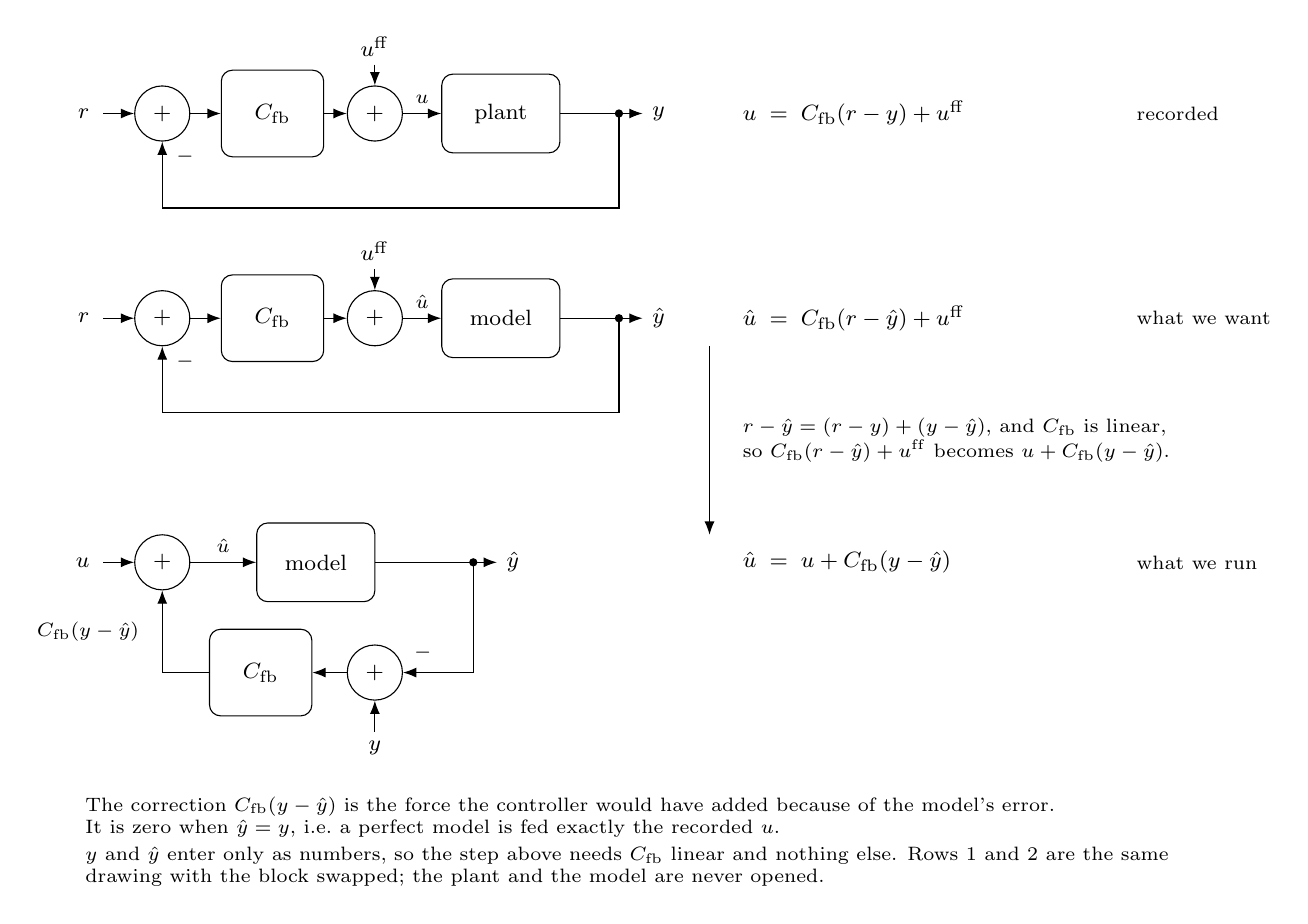
\begin{tikzpicture}[>=Latex, font=\footnotesize,
  block/.style={draw, rounded corners, minimum width=26mm, minimum height=12mm, align=center},
  rblock/.style={draw, rounded corners, minimum width=13mm, minimum height=11mm, align=center},
  small/.style={draw, rounded corners, minimum width=15mm, minimum height=10mm, align=center},
  sum/.style={draw, circle, minimum size=7mm, inner sep=0pt},
  jn/.style={circle, fill, minimum size=3pt, inner sep=0pt}]

% =================================================================================
% ROW 1: the machine
% =================================================================================
\node[sum]    (e1) at (0.35,0) {$+$};
\node[rblock] (c1) at (1.75,0) {$C_{\mathrm{fb}}$};
\node[sum]    (f1) at (3.05,0) {$+$};
\node[small]  (p1) at (4.65,0) {plant};

\node[left] at (-0.45,0) {$r$};
\draw[->] (-0.40,0) -- (e1.west);
\node at (3.05,0.85) {$u^{\mathrm{ff}}$};
\draw[->] (3.05,0.62) -- (f1.north);
\draw[->] (e1.east) -- (c1.west);
\draw[->] (c1.east) -- (f1.west);
\draw[->] (f1.east) -- (p1.west) node[pos=0.5,above]{\scriptsize $u$};
\draw[->] (p1.east) -- (6.45,0) node[right]{$y$};
\node[jn] at (6.15,0) {};
\draw[-]  (6.15,0) -- (6.15,-1.20) -- (0.35,-1.20);
\draw[->] (0.35,-1.20) -- (e1.south);
\node[font=\scriptsize] at (0.64,-0.55) {$-$};

% =================================================================================
% ROW 2: the same drawing, model in place of the plant
% =================================================================================
\node[sum]    (e2) at (0.35,-2.60) {$+$};
\node[rblock] (c2) at (1.75,-2.60) {$C_{\mathrm{fb}}$};
\node[sum]    (f2) at (3.05,-2.60) {$+$};
\node[small]  (p2) at (4.65,-2.60) {model};

\node[left] at (-0.45,-2.60) {$r$};
\draw[->] (-0.40,-2.60) -- (e2.west);
\node at (3.05,-1.75) {$u^{\mathrm{ff}}$};
\draw[->] (3.05,-1.98) -- (f2.north);
\draw[->] (e2.east) -- (c2.west);
\draw[->] (c2.east) -- (f2.west);
\draw[->] (f2.east) -- (p2.west) node[pos=0.5,above]{\scriptsize $\hat u$};
\draw[->] (p2.east) -- (6.45,-2.60) node[right]{$\hat y$};
\node[jn] at (6.15,-2.60) {};
\draw[-]  (6.15,-2.60) -- (6.15,-3.80) -- (0.35,-3.80);
\draw[->] (0.35,-3.80) -- (e2.south);
\node[font=\scriptsize] at (0.64,-3.15) {$-$};

% =================================================================================
% ROW 3: what we run
% =================================================================================
\node[sum]   (u3) at (0.35,-5.70) {$+$};
\node[small] (p3) at (2.30,-5.70) {model};
\node[sum]   (e3) at (3.05,-7.10) {$+$};
\node[rblock](c3) at (1.60,-7.10) {$C_{\mathrm{fb}}$};

\node[left] at (-0.45,-5.70) {$u$};
\draw[->] (-0.40,-5.70) -- (u3.west);
\draw[->] (u3.east) -- (p3.west) node[pos=0.5,above]{\scriptsize $\hat u$};
\draw[->] (p3.east) -- (4.60,-5.70) node[right]{$\hat y$};
\node[jn] at (4.30,-5.70) {};
\draw[-]  (4.30,-5.70) -- (4.30,-7.10);
\draw[->] (4.30,-7.10) -- (e3.east);
\node[font=\scriptsize] at (3.66,-6.85) {$-$};
\node[below] at (3.05,-7.85) {$y$};
\draw[->] (3.05,-7.85) -- (e3.south);
\draw[->] (e3.west) -- (c3.east);
\draw[-]  (c3.west) -- (0.35,-7.10);
\draw[->] (0.35,-7.10) -- (u3.south);
\node[anchor=east, font=\scriptsize] at (0.18,-6.58) {$C_{\mathrm{fb}}(y-\hat y)$};

% =================================================================================
% the three lines
% =================================================================================
\node[anchor=west] at (7.60,0)     {$u \;=\; C_{\mathrm{fb}}(r-y) + u^{\mathrm{ff}}$};
\node[anchor=west] at (7.60,-2.60) {$\hat u \;=\; C_{\mathrm{fb}}(r-\hat y) + u^{\mathrm{ff}}$};
\node[anchor=west] at (7.60,-5.70) {$\hat u \;=\; u + C_{\mathrm{fb}}(y-\hat y)$};

\node[anchor=west, font=\scriptsize] at (12.60,0)     {recorded};
\node[anchor=west, font=\scriptsize] at (12.60,-2.60) {what we want};
\node[anchor=west, font=\scriptsize] at (12.60,-5.70) {what we run};

\draw[->] (7.30,-2.95) -- (7.30,-5.35);
\node[anchor=west, align=left, font=\scriptsize] at (7.60,-4.15)
  {$r-\hat y=(r-y)+(y-\hat y)$, and $C_{\mathrm{fb}}$ is linear,\\
   so $C_{\mathrm{fb}}(r-\hat y)+u^{\mathrm{ff}}$ becomes $u+C_{\mathrm{fb}}(y-\hat y)$.};

% =================================================================================
\node[anchor=north west, align=left, font=\scriptsize] at (-0.75,-8.55)
  {The correction $C_{\mathrm{fb}}(y-\hat y)$ is the force the controller would have added
   because of the model's error.\\
   It is zero when $\hat y=y$, i.e.\ a perfect model is fed exactly the recorded $u$.\\[2pt]
   $y$ and $\hat y$ enter only as numbers, so the step above needs $C_{\mathrm{fb}}$ linear and
   nothing else. Rows 1 and 2 are the same\\
   drawing with the block swapped; the plant and the model are never opened.};

\end{tikzpicture}
\end{document}
